\documentclass[11pt,a4paper]{article}

% --- Paketler ---
\usepackage[utf8]{inputenc}
\usepackage[T1]{fontenc}
\usepackage[provide=*,turkish]{babel}
\usepackage[margin=2.5cm]{geometry}
\usepackage{amsmath,amssymb,amsfonts}
\usepackage{graphicx}
\usepackage{booktabs}
\usepackage{longtable}
\usepackage{array}
\usepackage{multirow}
\usepackage{xcolor}
\usepackage{hyperref}
\usepackage{enumitem}
\usepackage{titlesec}
\usepackage{fancyhdr}
\usepackage{tcolorbox}
\usepackage{listings}
\usepackage{caption}
\usepackage{tikz}
\usetikzlibrary{shapes.geometric,arrows.meta,positioning,fit,backgrounds}

% --- Renk tanımları ---
\definecolor{primary}{RGB}{0,90,170}
\definecolor{accent}{RGB}{200,80,40}
\definecolor{boxgray}{RGB}{245,245,245}
\definecolor{success}{RGB}{40,140,60}
\definecolor{warning}{RGB}{200,140,0}
\definecolor{danger}{RGB}{180,40,40}

% --- Hyperref ayarları ---
\hypersetup{
    colorlinks=true,
    linkcolor=primary,
    urlcolor=primary,
    citecolor=accent,
    pdftitle={Otonom Güneş Takip ve Parazitik Enerji Analiz Sistemi},
    pdfauthor={Proje Ekibi}
}

% --- Başlık formatları ---
\titleformat{\section}{\Large\bfseries\color{primary}}{\thesection.}{0.6em}{}
\titleformat{\subsection}{\large\bfseries\color{primary!85}}{\thesubsection.}{0.5em}{}
\titleformat{\subsubsection}{\normalsize\bfseries\color{accent}}{\thesubsubsection.}{0.4em}{}

% --- Header/Footer ---
\pagestyle{fancy}
\fancyhf{}
\fancyhead[L]{\small\textit{Solar Tracker Projesi}}
\fancyhead[R]{\small\thepage}
\renewcommand{\headrulewidth}{0.4pt}

% --- Özel kutular ---
\newtcolorbox{infobox}[1][]{
    colback=primary!5,
    colframe=primary,
    fonttitle=\bfseries,
    title=#1,
    boxrule=0.8pt,
    arc=2pt
}

\newtcolorbox{warnbox}[1][]{
    colback=warning!8,
    colframe=warning!80!black,
    fonttitle=\bfseries,
    title=#1,
    boxrule=0.8pt,
    arc=2pt
}

\newtcolorbox{successbox}[1][]{
    colback=success!8,
    colframe=success!70!black,
    fonttitle=\bfseries,
    title=#1,
    boxrule=0.8pt,
    arc=2pt
}

\newtcolorbox{dangerbox}[1][]{
    colback=danger!8,
    colframe=danger!70!black,
    fonttitle=\bfseries,
    title=#1,
    boxrule=0.8pt,
    arc=2pt
}

% --- Liste ayarları ---
\setlist[itemize]{leftmargin=*,topsep=2pt,itemsep=1pt}
\setlist[enumerate]{leftmargin=*,topsep=2pt,itemsep=1pt}

% --- Code listing stili ---
\lstdefinestyle{mystyle}{
    backgroundcolor=\color{boxgray},
    basicstyle=\ttfamily\small,
    breaklines=true,
    frame=single,
    framesep=4pt,
    rulecolor=\color{gray!40}
}
\lstset{style=mystyle}

% =========================================================
\begin{document}

% --- KAPAK ---
\begin{titlepage}
\centering
\vspace*{2cm}

{\color{primary}\rule{\textwidth}{1.5pt}}
\vspace{0.5cm}

{\Huge\bfseries Çift İşlemcili Otonom Güneş Takip ve\\[0.3cm] Parazitik Enerji Analiz Sistemi\par}
\vspace{0.5cm}

{\Large\itshape Donanım Mimarisi, Termal Yönetim ve\\Akademik Deney Tasarımı\par}
\vspace{0.3cm}
{\color{primary}\rule{\textwidth}{1.5pt}}

\vfill

\begin{tcolorbox}[colback=boxgray,colframe=primary,arc=4pt,width=0.85\textwidth]
\centering
\textbf{Proje Hipotezi:}\\[0.3cm]
\textit{Aktif takip algoritması ve akıllı petal kontrolü sayesinde, küçük ölçekli (sub-50W) bir güneş takip sistemi, parazitik tüketimi düşürerek sabit eğimli referans sisteme kıyasla net pozitif enerji kazancı sağlayabilir.}
\end{tcolorbox}

\vfill

\begin{tabular}{rl}
\textbf{Doküman Versiyonu:} & v1.0 \\
\textbf{Tarih:} & \today \\
\textbf{Kontrolcü:} & STM32 Nucleo-G431KB \\
\textbf{Veri Toplayıcı:} & ESP32-WROOM-32 \\
\textbf{Panel Konfigürasyonu:} & 4 $\times$ (20$\times$20 cm) $\approx$ 16--20 W \\
\textbf{Hedef Çalışma Süresi:} & $\geq$ 10 saat otonom \\
\end{tabular}

\vspace{1cm}
\end{titlepage}

% --- İçindekiler ---
\tableofcontents
\newpage

% =========================================================
\section{Yönetici Özeti}

Bu doküman, küçük ölçekli (4 panel, $\sim$20 W toplam) bir güneş takip sisteminin tam donanım mimarisini, termal yönetim stratejisini ve deney metodolojisini sunar. Projenin bilimsel özgünlüğü, sıradan bir ``tracker çalışıyor'' demonstrasyonunun ötesine geçerek; sistemin kendi parazitik tüketimini hassas ölçüm ile karakterize edip, takip algoritmasının sağladığı ek üretim ile karşılaştırarak \textbf{net enerji kazancı (E\textsubscript{net})} hipotezini test etmesidir.

\begin{infobox}[Temel Tasarım Kararları]
\begin{itemize}
    \item \textbf{Çift işlemcili mimari:} STM32G431KB (kontrol/hareket) + ESP32 (veri/iletişim) ayrımı; gerçek zamanlı kontrol döngüsünün veri kaydı kaynaklı gecikmelerden izole edilmesi.
    \item \textbf{Yedi noktada akım/gerilim ölçümü:} 6$\times$INA226 ile panel-bazlı üretim, MPPT çıkışı ve parazitik tüketim eş zamanlı izleme.
    \item \textbf{Çok katmanlı termal izleme:} Panel (4$\times$DS18B20), batarya (NTC) ve muhafaza içi (BME280 opsiyonel) sıcaklık karakterizasyonu.
    \item \textbf{Veri bütünlüğü garantisi:} DS3231 RTC + microSD + süper-kapasitör destekli güvenli yazma protokolü.
\end{itemize}
\end{infobox}

% =========================================================
\section{Sistem Mimarisi}

\subsection{Üç Katmanlı Yapı}

Sistem, sorumlulukların net olarak ayrıldığı üç fonksiyonel katmana bölünmüştür:

\begin{table}[h]
\centering
\renewcommand{\arraystretch}{1.3}
\begin{tabular}{|p{3cm}|p{4cm}|p{7cm}|}
\hline
\rowcolor{primary!15}
\textbf{Katman} & \textbf{Donanım} & \textbf{Görev} \\
\hline
1: Karar \& Hareket & STM32 Nucleo-G431KB & 4$\times$LDR okuma, FSM tabanlı takip algoritması, motor sürücü PWM çıkışı, sonsuz vida konum kontrolü \\
\hline
2: Veri Merkezi & ESP32-WROOM-32 & 6$\times$INA226 I2C okuma, panel/batarya/muhafaza sıcaklık verisi, RTC zaman damgası, microSD kayıt, UART üzerinden STM32 ile haberleşme \\
\hline
3: İzleme \& Yedek & MATLAB / PC & USB seri port üzerinden canlı veri akışı, gerçek zamanlı grafik (üretim vs.\ tüketim), bilgisayar diskine yedek kayıt \\
\hline
\end{tabular}
\caption{Üç katmanlı sistem mimarisi ve sorumluluk dağılımı.}
\end{table}

\textbf{Tasarım gerekçesi:} Kontrol ve veri toplama görevlerinin tek bir mikroişlemciye yüklenmesi, SD kart yazma gecikmelerinin (10-50 ms) PID döngüsünü bozma riskini doğurur. Çift işlemcili ayrım bu riski tamamen ortadan kaldırır ve katmanlar bağımsız olarak debug edilebilir hale gelir.

\subsection{Veri Akış Diyagramı}

\begin{figure}[h]
\centering
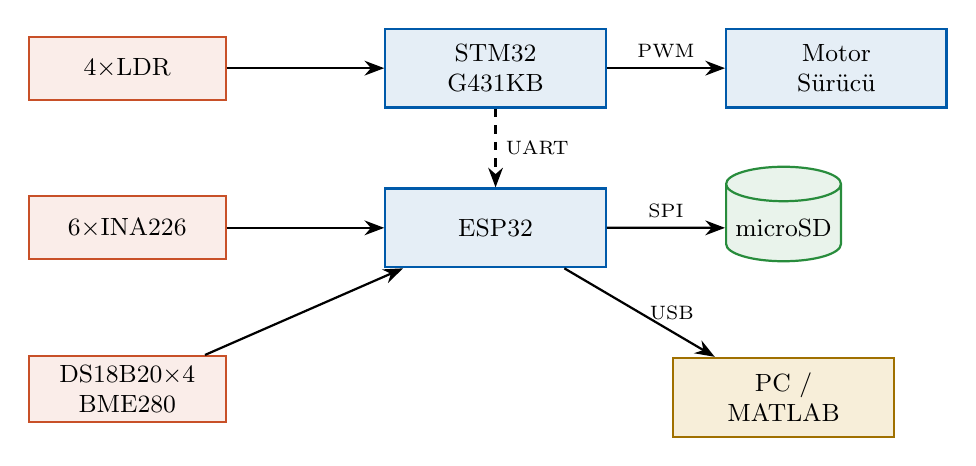
\begin{tikzpicture}[
    node distance=1.2cm and 1.5cm,
    block/.style={rectangle, draw=primary, fill=primary!10, thick, minimum width=2.8cm, minimum height=1cm, align=center, font=\small},
    sensor/.style={rectangle, draw=accent, fill=accent!10, thick, minimum width=2.5cm, minimum height=0.8cm, align=center, font=\small},
    storage/.style={cylinder, shape border rotate=90, draw=success, fill=success!10, thick, aspect=0.3, minimum height=1.2cm, align=center, font=\small},
    arrow/.style={-{Stealth[length=2.5mm]}, thick}
]

% Sensors
\node[sensor] (ldr) {4$\times$LDR};
\node[sensor, below=of ldr] (ina) {6$\times$INA226};
\node[sensor, below=of ina] (temp) {DS18B20$\times$4\\BME280};

% Controllers
\node[block, right=2cm of ldr] (stm) {STM32\\G431KB};
\node[block, right=2cm of ina] (esp) {ESP32};

% Outputs
\node[block, right=of stm] (motor) {Motor\\Sürücü};
\node[storage, right=of esp] (sd) {microSD};
\node[block, below=of sd, fill=warning!15, draw=warning!80!black] (pc) {PC /\\MATLAB};

% Arrows
\draw[arrow] (ldr) -- (stm);
\draw[arrow] (ina) -- (esp);
\draw[arrow] (temp) -- (esp);
\draw[arrow] (stm) -- node[above, font=\scriptsize] {PWM} (motor);
\draw[arrow] (esp) -- node[above, font=\scriptsize] {SPI} (sd);
\draw[arrow] (esp) -- node[right, font=\scriptsize] {USB} (pc);
\draw[arrow, dashed] (stm) -- node[right, font=\scriptsize, pos=0.5] {UART} (esp);

\end{tikzpicture}
\caption{Sistem veri akışı: Sensör girişlerinden depolama/izleme katmanlarına.}
\end{figure}

% =========================================================
\section{Donanım Bileşen Listesi (BOM)}

\subsection{Karar Hiyerarşisi: Olmazsa Olmaz / Önerilen / Çıkarılan}

Bütçe optimizasyonu sürecinde, her bileşen üç kategoride değerlendirilmiştir.

\subsection{Çekirdek Bileşenler (Olmazsa Olmaz)}

\begin{longtable}{|p{4.5cm}|p{1.3cm}|p{1.5cm}|p{6cm}|}
\hline
\rowcolor{primary!15}
\textbf{Bileşen} & \textbf{Adet} & \textbf{Maliyet (USD)} & \textbf{Gerekçe} \\
\hline
\endhead

STM32 Nucleo-G431KB & 1 & Mevcut & 170 MHz Cortex-M4 + FPU, motor kontrol için optimize G4 serisi (HRTIM, CORDIC, FMAC). Hareket katmanı kontrolcüsü. \\
\hline
ESP32-WROOM-32 DevKit & 1 & 5--8 & Dual-core 240 MHz, dahili WiFi/BT, FreeRTOS desteği. Veri toplama ve iletişim katmanı. \\
\hline
INA226 Akım/Gerilim Sensörü & 6 & 18--24 & Yüksek hassasiyetli I2C tabanlı güç ölçümü. Panel-bazlı (4) + MPPT çıkışı (1) + ana besleme/parazitik (1). Adresleme A0/A1 pinleriyle. \\
\hline
LDR + 10k pull-down & 4 & 2 & Mevcut algoritma için ışık yönü tespiti. \\
\hline
DS3231 RTC modülü & 1 & 3 & Pil yedekli gerçek zamanlı saat. ±2 ppm hassasiyet, ESP32'nin kendi zamanı güç kesintisinde kaybolur. \\
\hline
SPI MicroSD modülü + 32GB SD & 1 & 10 & Veri loglama. Sıradan SanDisk Ultra yeterli (kısa-orta vadeli deney). \\
\hline
CN3791 MPPT modülü & 1 & 5--8 & Panel--batarya gerilim eşleşmesi ve maksimum güç noktası takibi. Telemetri yok ama INA226'lar bu boşluğu dolduruyor. \\
\hline
LiFePO4 12V 7Ah batarya & 1 & 60--80 & Termal güvenlik (kaçak sıcaklığı $\sim$270°C), uzun çevrim ömrü ($\geq$3000), outdoor için ideal. \\
\hline
Pololu D24V22F5 buck (5V 2A) & 1 & 15 & Kontrolcü ve sensör hattı için temiz 5V. LM2596 gibi ucuz alternatifler INA226 ölçümlerini bozar. \\
\hline
Motor Sürücü (BTS7960 veya DRV8833) & 1--2 & 5--10 & Pan/tilt motor sürümü. Sayı motor sayısına bağlı. \\
\hline
Süper kapasitör (5.5V 1F) + 1N5817 & 1 & 4 & Power-loss durumunda son SD yazımının tamamlanması. \\
\hline
\end{longtable}

\textbf{Çekirdek alt-toplam: $\sim$130--165 USD} (LiFePO4 dahil)

\subsection{Termal İzleme (Sadeleştirilmiş)}

\begin{longtable}{|p{4.5cm}|p{1.3cm}|p{1.5cm}|p{6cm}|}
\hline
\rowcolor{primary!15}
\textbf{Bileşen} & \textbf{Adet} & \textbf{Maliyet (USD)} & \textbf{Gerekçe} \\
\hline
\endhead

DS18B20 (kapsüllü, su geçirmez) & 4 & 10 & Panel arka yüzeyi sıcaklığı. 1-Wire ile tek pinden 4 sensör. Hipotezi destekleyen ölçüm verisi. \\
\hline
10K NTC termistör & 1 & 1 & Batarya yüzey sıcaklığı (güvenlik kritik, 60°C üstüne çıkmamalı). STM32 ADC'sine bağlı. \\
\hline
Arctic MX-4 termal macun & 1 & 5 & DS18B20'leri panel arkasına yapıştırma. Yalnız bant kullanılırsa 5--10°C ölçüm hatası oluşur. \\
\hline
5V 40 mm fan + IRF540 MOSFET & 1 & 5 & 50°C eşik aşıldığında devreye giren aktif soğutma. Histerezis: 50°C aç, 42°C kapat. \\
\hline
\end{longtable}

\textbf{Termal alt-toplam: $\sim$21 USD}

\subsection{Muhafaza ve Kablolama}

\begin{longtable}{|p{4.5cm}|p{1.3cm}|p{1.5cm}|p{6cm}|}
\hline
\rowcolor{primary!15}
\textbf{Bileşen} & \textbf{Adet} & \textbf{Maliyet (USD)} & \textbf{Gerekçe} \\
\hline
\endhead

IP65 polikarbonat kutu (beyaz) & 1 & 10--15 & Beyaz renk: güneş altında siyah kutuya göre $\sim$20°C daha düşük iç sıcaklık. \\
\hline
Kablo rakoru (PG7/PG9 IP68) & 2--3 & 3 & Sızdırmaz kablo girişi. \\
\hline
GoreTex breather valve & 1 & 5 (ops.) & Basınç dengesi + nem önleme. Eğer muhafaza tamamen sızdırmaz ve sürekli outdoor ise kritik; kısa süreli deney için atlanabilir. \\
\hline
JST konnektör seti & 1 set & 3 & Sökülebilirlik. Sahada hatalı bileşen değişimini hızlandırır. \\
\hline
22 AWG silikon kablo + 16 AWG güç kablosu & -- & 5--10 & Sürekli outdoor için silikon (PVC güneşte sertleşir). \\
\hline
4.7k pull-up direnç (I2C, 1-Wire için) & 8--10 & 1 & Kütüphanelerin doğru çalışması için zorunlu. \\
\hline
\end{longtable}

\textbf{Muhafaza/kablo alt-toplam: $\sim$27--37 USD}

\subsection{Çıkarılan Bileşenler ve Gerekçeleri}

Aşağıdaki bileşenler, prototip aşamasında \textbf{maliyet/fayda dengesi açısından} listeden çıkarılmıştır. İleride akademik yayın hedeflenirse eklenmeli.

\begin{longtable}{|p{4cm}|p{2cm}|p{8cm}|}
\hline
\rowcolor{danger!15}
\textbf{Çıkarılan Bileşen} & \textbf{Tasarruf (USD)} & \textbf{Gerekçe \& Sonuç} \\
\hline
\endhead

AS5600 manyetik encoder & 6 & Mevcut algoritma encoder kullanmıyor (LDR-based feedback). Pozisyon doğruluğu LDR ile sağlanıyor. \\
\hline
MPU6050 / BNO055 IMU & 12 & Algoritma absolute açı bilgisine ihtiyaç duymuyor. \\
\hline
FRAM (MB85RC256V) & 4 & Süper kapasitör + SD kart kombinasyonu yeterli güvenilirlik. \\
\hline
Pyranometer (Apogee SP-110) & 150--180 & \textit{Akademik yayın} için kritik (irradyans normalizasyonu). Prototip aşamasında atlanabilir; ileride eklenmeli. \\
\hline
Referans sabit panel sistemi & 200--250 & Eş zamanlı karşılaştırma için gerekli. Şu an sadece tracker karakterizasyonu yapılıyor. \\
\hline
BME280 (muhafaza içi nem) & 5 & Sızdırmaz muhafaza ve breather valve ile yoğuşma riski yönetilebilir. \\
\hline
Endüstriyel grade microSD & 10 & Sıradan kart ile aylık deneyler güvenli; sadece sürekli (yıllık) loglama için gerekli. \\
\hline
\end{longtable}

\subsection{Bütçe Özeti}

\begin{table}[h]
\centering
\renewcommand{\arraystretch}{1.3}
\begin{tabular}{|l|r|}
\hline
\rowcolor{primary!15}
\textbf{Kategori} & \textbf{Maliyet (USD)} \\
\hline
Çekirdek elektronik (LiFePO4 ile) & 130--165 \\
\hline
Termal izleme (sadeleştirilmiş) & 21 \\
\hline
Muhafaza ve kablolama & 27--37 \\
\hline
\textbf{Prototip Toplam} & \textbf{180--225} \\
\hline
\hline
Akademik genişletme (pyranometer + referans) & +350--430 \\
\hline
\textbf{Tam Akademik Toplam} & \textbf{530--655} \\
\hline
\end{tabular}
\caption{Aşamalı bütçe planı: prototip $\rightarrow$ akademik yayın hedefi.}
\end{table}

% =========================================================
\section{Donanım Mimarisi Detayları}

\subsection{Blok 1: Enerji Üretim ve Yönetim}

\subsubsection{Panel Konfigürasyonu}

4 adet 20$\times$20 cm panel, ortalama 5 W $@$ 6 V çıkışlı varsayılır. Önerilen topoloji: \textbf{paralel bağlantı $@$ 6 V nominal}, toplam 20 W max. Gerekçe: yüksek voltaj/düşük akım yerine düşük voltaj/yüksek akım, MPPT modülü ve kablolama için daha güvenli. Her panelin çıkışı bir INA226 üzerinden geçer; bu sayede mismatch loss (panel-arası uyumsuzluk kaybı) gerçek zamanlı tespit edilir.

\subsubsection{Güç Bütçesi Hesabı}

Saha koşullarında günlük tipik değerler:

\begin{align}
E_{\text{üretim}} &= P_{\text{ortalama}} \times t_{\text{etkin güneş}} \nonumber \\
                  &= 12\,\text{W} \times 5.5\,\text{h} = 66\,\text{Wh/gün}
\end{align}

\begin{align}
E_{\text{parazitik}} &= P_{\text{kontrol}} \cdot t + E_{\text{motor}} + E_{\text{soğutma}} \nonumber \\
                     &\approx 1.0\,\text{W} \times 10\,\text{h} + 1\,\text{Wh} + 3\,\text{Wh} \nonumber \\
                     &\approx 14\,\text{Wh/gün}
\end{align}

\begin{align}
E_{\text{net}} = E_{\text{üretim}} - E_{\text{parazitik}} \approx 52\,\text{Wh/gün}
\end{align}

\begin{warnbox}[Marjinal Denge Uyarısı]
Tracker kazancı (sabit sisteme göre) tipik olarak \%15--30, yani ek 10--20 Wh/gün. Parazitik tüketim ($\sim$14 Wh) bu kazanca \textbf{çok yakın} mertebede. Bu nedenle:
\begin{itemize}
    \item Algoritmanın enerji-bilinçli olması (event-triggered control, deadband) kritik.
    \item INA226 ölçümlerinin hassasiyeti, hipotezin test edilebilmesi için doğrudan belirleyici.
    \item Yayın hedefliyorsanız eş zamanlı sabit referans \textbf{olmazsa olmaz}.
\end{itemize}
\end{warnbox}

\subsection{Blok 2: Kontrol ve Hareket}

\subsubsection{STM32 Nucleo-G431KB Seçim Gerekçesi}

\begin{infobox}[STM32G431KB Avantajları]
\begin{itemize}
    \item 170 MHz Cortex-M4 + FPU --- floating point PID hesaplamaları
    \item HRTIM (High-Resolution Timer) --- motor kontrol için endüstri standardı
    \item CORDIC \& FMAC donanım hızlandırıcıları --- trigonometrik ve matris işlemleri
    \item 4$\times$ op-amp, 7$\times$ komparatör --- analog ön-işleme
    \item 12-bit ADC, 5 Msps --- LDR okumalarında yüksek hız
    \item G4 ailesi: motor kontrol \& dijital güç için \textit{özel olarak} tasarlanmış
\end{itemize}
\end{infobox}

\textbf{Kısıt:} Nucleo-32 form faktörü = sadece 32 pin. Sistemde toplam aktüatör sayısına bağlı olarak pin yetmezlik riski. Eğer pan-tilt + petal toplam motor sayısı $\geq 4$ ise, ya I/O expander (PCF8574) eklenecek ya da NUCLEO-G474RE'ye geçilecek.

\subsubsection{Motor Sürücü Seçimi}

\begin{itemize}
    \item \textbf{Pan-tilt için DC motor + sonsuz vida:} Sonsuz vidanın self-locking özelliği sayesinde motor durduğunda enerji tüketimi sıfır. PWM oranı $\rightarrow$ hız kontrolü.
    \item \textbf{BTS7960:} 43A pik kapasite (sistemin çok üstünde, ama dayanıklılık avantajı). Ucuz, yaygın. Çift modül = pan + tilt.
    \item \textbf{DRV8833 (alternatif):} Düşük güçlü motorlarda tek modülde 2 motor sürer, $\sim$3 USD. Petal aktüatörleri için ideal.
    \item \textbf{Petal motorları servo ise:} STM32 PWM pininden doğrudan sürülür, ek sürücü gerekmez.
\end{itemize}

\subsection{Blok 3: Sensör ve Ölçüm}

\subsubsection{INA226 Adresleme Şeması}

I2C üzerinde 6 adet INA226'nın eşzamanlı çalışması için A0/A1 pinleri ile farklı adresler:

\begin{table}[h]
\centering
\begin{tabular}{|c|c|c|p{6cm}|}
\hline
\rowcolor{primary!15}
\textbf{INA226 \#} & \textbf{A1, A0} & \textbf{Adres (7-bit)} & \textbf{Görev} \\
\hline
1 & GND, GND & 0x40 & Panel 1 çıkışı \\
2 & GND, VS  & 0x41 & Panel 2 çıkışı \\
3 & GND, SDA & 0x42 & Panel 3 çıkışı \\
4 & GND, SCL & 0x43 & Panel 4 çıkışı \\
5 & VS, GND  & 0x44 & MPPT çıkışı (toplam üretim) \\
6 & VS, VS   & 0x45 & Sistem ana besleme (parazitik) \\
\hline
\end{tabular}
\caption{INA226 I2C adresleme planı.}
\end{table}

\textbf{Shunt direnç dikkat:} Standart modüllerde 100m$\Omega$ shunt vardır (panel ölçümleri için uygun, 0--800 mA). Batarya/ana besleme hattında ise akım pikleri 1A'i aşabilir; bu noktadaki INA226'nın shunt'ı \textbf{10m$\Omega$} ile değiştirilmeli.

\subsubsection{LDR Okuma Devresi}

Klasik gerilim bölücü:
\begin{equation}
V_{\text{ADC}} = V_{\text{ref}} \cdot \frac{R_{\text{pull-down}}}{R_{\text{LDR}} + R_{\text{pull-down}}}
\end{equation}

$R_{\text{pull-down}} = 10\,\text{k}\Omega$ değeri, tipik LDR'nin orta ışık seviyesinde dengeli okuma vermesi için seçilmiştir. STM32'nin ADC'si 12-bit (4096 seviye), $V_{\text{ref}} = 3.3$ V.

\subsection{Blok 4: Veri Toplama ve Depolama}

\subsubsection{CSV Log Formatı}

Önerilen satır formatı (saniyede bir):

\begin{lstlisting}
timestamp,P1_V,P1_I,P2_V,P2_I,P3_V,P3_I,P4_V,P4_I,Vbat,Ibat,
Vmppt,Imppt,Vsys,Isys,T_p1,T_p2,T_p3,T_p4,T_bat,T_enc,
LDR1,LDR2,LDR3,LDR4,motor_state,fan_state
\end{lstlisting}

Tipik satır boyutu: $\sim$200 byte. 10 saatlik (36000 satır) log: $\sim$7 MB. 32 GB kart ile teorik olarak \textit{yıllarca} sürekli kayıt mümkün.

\subsubsection{Olay Tabanlı (Event-Driven) Log}

Standart 1 Hz log'a ek olarak, kritik olaylar ayrı dosyaya yazılır:

\begin{lstlisting}
2026-05-07 14:23:15, EVENT, BATTERY_TEMP_WARN, 55.2C
2026-05-07 14:23:18, EVENT, FAN_ON, enc_temp=51.3C
2026-05-07 14:31:02, EVENT, FAN_OFF, enc_temp=41.8C
2026-05-07 15:02:44, EVENT, PANEL3_HOTSPOT, T=68C, others=52C
\end{lstlisting}

\subsubsection{Güvenli Yazma Protokolü}

\begin{enumerate}
    \item Her dakika \texttt{flush()} çağır --- buffer'daki veriyi diske aktar.
    \item Her saat dosyayı \texttt{close()} edip yeni dosya aç.
    \item Süper kapasitör (5.5V 1F) ESP32'yi 2-3 sn besler --- ani kesintide son yazma tamamlanır.
    \item Power-loss tespiti: STM32 batarya gerilimini izler, eşik altında \texttt{POWER\_FAIL} sinyali gönderir, ESP32 acil kapanış sekansına girer.
\end{enumerate}

\subsection{Blok 5: Termal Yönetim}

\subsubsection{4 Katmanlı Termal Strateji}

\textbf{Katman 1 --- Panel Sıcaklık İzleme:} 4$\times$DS18B20, panel arka yüzey merkezine termal macun + Kapton bant ile yapıştırma. Üstten beyaz reflektif bant ile direkt ışınım korumalı. 1-Wire bus üzerinde tek pinden okunur.

\textbf{Katman 2 --- Muhafaza Termal Tasarımı:} Beyaz IP65 kutu (siyaha göre $\sim$20°C avantaj). GoreTex breather valve. 50°C eşikte aktif fan (histerezis: 50/42°C).

\textbf{Katman 3 --- Bileşen-Seviye Koruma:} Batarya 10K NTC ile, $T > 60$°C'de şarj kesimi. Motor sürücüde küçük heatsink. MPPT gölgeli yere monte.

\textbf{Katman 4 --- Olay Loglama:} Her termal eşik geçişi event log'a yazılır. Sıcaklık-üretim korelasyonu post-analiz için.

\subsubsection{Sıcaklık-Verim İlişkisi}

Silikon panel için tipik sıcaklık katsayısı:
\begin{equation}
\eta(T) = \eta_{\text{STC}} \cdot \left[1 + \alpha_P (T - 25\,°\text{C})\right]
\end{equation}

$\alpha_P \approx -0.004$ ile $-0.005$ /°C. Yani 65°C'de panel verimi $\sim$\%16-20 düşer. Bu kayıp, projenin termal verisinin akademik değerini doğrudan oluşturur.

% =========================================================
\section{Aşamalı Uygulama Planı}

\begin{table}[h]
\centering
\renewcommand{\arraystretch}{1.4}
\begin{tabular}{|c|p{4cm}|p{8cm}|}
\hline
\rowcolor{primary!15}
\textbf{Aşama} & \textbf{Hedef} & \textbf{Kabul Kriteri} \\
\hline
0 & Termal karakterizasyon & Tek panel + DS18B20 ile saatlik sıcaklık-irradyans verisi. \\
\hline
1 & ESP32 + RTC + 1$\times$INA226 + SD test & SD karta CSV satır yazma; dosya açma/kapama döngüsü stabil. \\
\hline
2 & Mekanik + STM32 FSM & LDR okuma, motor sürme, sonsuz vida hareket testi. Uyku moduna geçiş. \\
\hline
3 & UART entegrasyon (STM32 $\leftrightarrow$ ESP32) & Saniyede bir [açı, durum] verisi STM32'den ESP32'ye akıyor; ESP32 birleştirip kaydediyor. \\
\hline
4 & Tam sensör entegrasyonu & 6$\times$INA226 + 4$\times$DS18B20 + NTC tüm verileri tek CSV'de. \\
\hline
5 & Termal davranış testi (24 saat) & Lab koşullarında, fan döngüsü doğru çalışıyor; batarya $T < 50$°C kalıyor. \\
\hline
6 & Saha (10 saat outdoor) & Kesintisiz veri kaydı; veri kaybı $< \%0.1$. \\
\hline
7 & Veri analizi \& raporlama & Üretim, parazitik, net enerji grafikleri; sıcaklık-verim korelasyon analizi. \\
\hline
\end{tabular}
\caption{Aşamalı uygulama planı ve kabul kriterleri.}
\end{table}

% =========================================================
\section{Akademik Hipotez ve Deney Tasarımı}

\subsection{Hipotez Formülasyonu}

\begin{infobox}[Ana Hipotez (H1)]
Aktif takip + akıllı petal kontrolü kombinasyonu, sabit eğimli (fixed-tilt) referans sisteme kıyasla net pozitif enerji kazancı sağlar.
\[
E_{\text{net}}^{\text{tracker}} = E_{\text{üretim}}^{\text{tracker}} - E_{\text{parazitik}} > E_{\text{üretim}}^{\text{fixed}}
\]
\end{infobox}

\subsection{Literatürdeki Tartışma}

Tek eksen tracker'lar, sabit sisteme göre tipik \%15--30 ek üretim sağlar; iki eksenliler \%25--40 aralığında. Ancak \textbf{küçük ölçekli sistemlerde (<50 W)} parazitik tüketim bu kazancı yiyebilir. Bu nedenle ticari tracker'lar çoğunlukla 100 W ve üstü panellerle satılır. Senin projenin akademik fırsatı: \textit{algoritma optimizasyonu ile küçük sistemlerde de pozitif kazancın mümkün olduğunu göstermek.}

\subsection{Olası Sonuç Senaryoları}

\begin{table}[h]
\centering
\renewcommand{\arraystretch}{1.3}
\begin{tabular}{|p{2cm}|p{4cm}|p{8cm}|}
\hline
\rowcolor{primary!15}
\textbf{Senaryo} & \textbf{Sonuç} & \textbf{Akademik Değer} \\
\hline
A & $E_{\text{net}}^{\text{tracker}} > E_{\text{fixed}}$ & Hipotez doğrulanır. \textit{Yüksek değerli pozitif sonuç:} ``Küçük ölçekte algoritma ile pozitif kazanç mümkündür.'' Solar Energy / Energy Conversion and Management düzeyi yayın. \\
\hline
B & $E_{\text{net}}^{\text{tracker}} < E_{\text{fixed}}$ & Hipotez reddedilir. \textit{Hala değerli negatif sonuç:} ``Bu boyutta tracker haklı çıkmaz'' tezini sayısal kanıtla destekler. Etik açıdan paha biçilmez veri. \\
\hline
C & Koşullu sonuç & Bazı koşullarda kazanır, bazılarında kaybeder. Algoritma için \textit{mode-switching} mekanizması: parlak günde tracker, bulutluda fixed mode. Yenilikçi katkı. \\
\hline
\end{tabular}
\caption{Olası deney sonuçları ve akademik değerlendirme.}
\end{table}

\subsection{Metodolojik Gereksinimler (Akademik Yayın İçin)}

\begin{dangerbox}[Reviewer Tuzakları]
Aşağıdaki gereksinimler atlanırsa, hangi sonuç çıkarsa çıksın yayın \textbf{ilk turda reddedilir}:
\begin{itemize}
    \item \textbf{Eş zamanlı karşılaştırma:} Tracker ve fixed sistem aynı anda çalışmalı (farklı günlerde test geçerli değildir).
    \item \textbf{Optimal fixed eğim:} Referans sistem, konuma uygun yıllık optimal açıda olmalı (İstanbul için $\sim$35° güney).
    \item \textbf{Yeterli süre:} Minimum 30 gün, farklı hava koşulları kapsamı.
    \item \textbf{İrradyans normalizasyonu:} Pyranometer ile.
    \item \textbf{İstatistiksel analiz:} Paired t-test veya Wilcoxon, p-değeri ve effect size raporlama.
\end{itemize}
\end{dangerbox}

\subsection{Veri Analizi Yapısı}

Toplanan veriler şu analizleri mümkün kılar:

\begin{enumerate}
    \item \textbf{Birincil:} Net enerji kazancı dağılımı (tracker vs.\ fixed, eğer referans varsa).
    \item \textbf{İkincil --- Termal:} Panel sıcaklığı $\rightarrow$ verim regresyonu (lineer fit + $\alpha_P$ kestirimi).
    \item \textbf{İkincil --- Mismatch:} 4 panel arası üretim varyansı, gölgelenme tespiti.
    \item \textbf{İkincil --- Parazitik:} Motor hareketi sıklığı vs.\ enerji maliyeti, hareket başına net Wh.
    \item \textbf{Tertier:} Soğutma fanının net enerji etkisi (fan tüketimi vs.\ panel verim artışı).
\end{enumerate}

% =========================================================
\section{Risk Değerlendirmesi ve Azaltma}

\begin{longtable}{|p{4cm}|c|c|p{6cm}|}
\hline
\rowcolor{primary!15}
\textbf{Risk} & \textbf{Olasılık} & \textbf{Etki} & \textbf{Azaltma} \\
\hline
\endhead

SD kart bozulması & Orta & Yüksek & Süper kapasitör + güvenli yazma protokolü; günlük dosya rotasyonu. \\
\hline
Batarya termal kaçak & Düşük & Kritik & LiFePO4 + NTC monitör + 60°C'de şarj kesimi. \\
\hline
Pin yetersizliği (Nucleo-32) & Orta & Orta & PCF8574 I/O expander veya NUCLEO-G474RE'ye geçiş. \\
\hline
Yağmur/nem girişi & Orta & Yüksek & IP65 kutu + GoreTex valve + kablo rakorları. \\
\hline
Parazitik tüketim hipotezi yanlış çıkar & Orta & Düşük & Negatif sonuç da yayın değeri taşır (Senaryo B). \\
\hline
INA226 ölçüm hatası (gürültü) & Düşük & Orta & Pololu buck (LM2596 değil); sensör hatlarına ferrit boncuk. \\
\hline
10 saat hedefi karşılanmaz & Düşük & Düşük & Batarya kapasitesi 84 Wh, tüketim $<$15 Wh/gün $\Rightarrow$ \%5 derinlik deşarjı. \\
\hline
Yazılım kilitlenmesi & Orta & Orta & STM32 ve ESP32'de bağımsız watchdog (IWDG) etkin. \\
\hline
\end{longtable}

% =========================================================
\section{Tartışılması Gereken Açık Noktalar}

Donanım mimarisinin son haline gelmesi için aşağıdaki kararlar netleştirilmelidir:

\begin{enumerate}
    \item \textbf{Pan-tilt motor sayısı ve tipi.} 1 motor + diferansiyel mekanizma mı, yoksa 2 ayrı DC motor mu? Bu, motor sürücü sayısını ve pin bütçesini doğrudan belirler.
    \item \textbf{Petal aktüatörü.} Servo (PWM doğrudan), DC motor (ek sürücü), veya merkezi mekanizma (tek aktüatör)?
    \item \textbf{Kurulum kalıcılığı.} Sürekli outdoor mu, yoksa sadece deney sırasında dışarı mı çıkıyor? (LiFePO4 vs.\ SLA, IP65 derecesinin önemi.)
    \item \textbf{Akademik hedef.} Sadece prototip mi, yoksa sonradan referans sistem + pyranometer eklenecek mi? (Bütçe planlaması.)
    \item \textbf{Veri toplama süresi.} Tek 10 saatlik deney mi, yoksa sürekli aylar süren kayıt mı? (Industrial SD kart gerekliliği.)
\end{enumerate}

% =========================================================
\section{Sonuç ve Sonraki Adımlar}

Bu doküman, çekirdek prototip için \textbf{$\sim$180-225 USD bütçeyle} çalışan, akademik geçerliliği olan bir solar tracker sisteminin donanım mimarisini ortaya koymaktadır. Sistem; çift işlemcili ayrım, 6 noktalı güç ölçümü ve 4 katmanlı termal izleme ile sıradan tracker projelerinden ayrışır.

\textbf{Bir sonraki doküman versiyonu (v1.1) için planlanan eklemeler:}
\begin{itemize}
    \item Bağlantı şeması (KiCad veya Fritzing)
    \item STM32 pin atama tablosu (motor sayısı netleştikten sonra)
    \item ESP32 FreeRTOS task mimarisi
    \item Watchdog ve hata kurtarma akış şemaları
    \item İlk laboratuvar testi sonuçları
\end{itemize}

\vfill

\begin{center}
\rule{0.6\textwidth}{0.5pt}\\[0.3cm]
\textit{Doküman v1.0 --- \today}\\
\textit{Yaşayan doküman: her aşama tamamlandığında güncellenir.}
\end{center}

\end{document}
